\documentclass[a4paper, 12pt]{report}
\usepackage{graphicx}
\usepackage[swedish]{babel}
\usepackage[style=iso]{datetime2}
\usepackage{float}
\usepackage{caption}
	\captionsetup{width=.9\linewidth}
% \usepackage{subcaption,xcolor,lipsum}
\usepackage{verbatim}
% \usepackage{changepage}
\usepackage{amsmath}
\usepackage{amssymb}
\usepackage{microtype}
\usepackage{rotate}
\usepackage{siunitx}
\usepackage[backend=biber,sorting=none]{biblatex} %Imports biblatex package
\usepackage{tikz}
\usepackage[margin=1.2in]{geometry} %% 1.2 in
\usepackage{titlesec}
\usetikzlibrary{math, arrows.meta}
\addbibresource{references/references.bib}
\newcommand{\Lagr}{\mathcal{L}}
\usepackage[toc,page]{appendix}
\usepackage{subcaption}
\usepackage{changepage}
\usepackage{listings}
\usepackage{xcolor}

\newcommand*{\QED}{\hfill\ensuremath{\blacksquare}}

\setlength{\parindent}{0pt}
% men däremot lite mellanrum
\setlength{\parskip}{10pt}

\refstepcounter{chapter} % increment chapter counter manually

	\usepackage{hyperref}
		\hypersetup{
			colorlinks=true,
			linkcolor=black,
			filecolor=magenta,      
			urlcolor=cyan,
			citecolor=blue,
			pdftitle={Overleaf Example},
			pdfpagemode=FullScreen,
			}


\definecolor{codegreen}{rgb}{0,0.6,0}
\definecolor{codegray}{rgb}{0.5,0.5,0.5}
\definecolor{codepurple}{rgb}{0.58,0,0.82}
\definecolor{backcolour}{rgb}{0.95,0.95,0.92}

\lstdefinestyle{mystyle}{
    backgroundcolor=\color{backcolour},   
    commentstyle=\color{codegreen},
    keywordstyle=\color{magenta},
    numberstyle=\tiny\color{codegray},
    stringstyle=\color{codepurple},
    basicstyle=\ttfamily\footnotesize,
    breakatwhitespace=false,         
    breaklines=true,                 
    captionpos=b,                    
    keepspaces=true,                 
    numbers=left,                    
    numbersep=5pt,                  
    showspaces=false,                
    showstringspaces=false,
    showtabs=false,                  
    tabsize=2
}

\lstset{style=mystyle}

\graphicspath{{./images/}}

% Så att "Kapitel x" försvinner
% \titleformat{\chapter}
%   {\Large\bfseries} % format
%   {}                % label
%   {0pt}             % sep
%   {\huge}           % before-code

\usepackage{titlesec}

\titleformat{\chapter}[hang] % 'hang' makes the title appear on the same line
  {\normalfont\huge\bfseries} % Format of the whole title
  {\thechapter.} % Label (number + dot)
  {20pt} % Separation between number and title
  {\huge} % Code before the title

\titlespacing{\chapter}{0pt}{50pt}{40pt}

\begin{document}
\renewcommand{\abstractname}{Abstract}
\begin{titlepage}
	\centering
	\includegraphics[width=0.3\textwidth]{europaskolan.png}\par\vspace{1cm}
	{\LARGE \textsc{Europaskolan Strängnäs}\par}
	\vspace{1cm}
	{\Large \textsc{Gymnasiearbete}\par}
	\vspace{1.5cm}
	{\huge\bfseries Dubbelpendeln och kaosteori \par}
	\vspace{2cm}
	{\Large\itshape Oscar Landberg \\
		KFSCI23b\par}
	\vfill
	Handledare:\par
    \vspace{-1.5mm}
	Erik Waltersson

	\vfill

	%% nedre delen av framsidan
	{\large Första utkast inlämnat: \today}
\end{titlepage}

\begin{abstract}
    Here is my Triangle. 
\end{abstract}
\pagenumbering{gobble}
\tableofcontents
\chapter*{Inledning}

\section{Bakgrund}
Pendeln är något som alltid har fascinerat mänskligheten genom tiderna. Redan under det första århundradet lyckades de gamla kineserna att utveckla en seismograf med hjälp av pendeln, vars funktion funktion var att aktivera ett säkerhetssystem vid jordbävningar \cite{book:china_history}. Inte minst används också pendlar än idag; Mora-klockors tidhållning bygger på en svängande pendel, medan den klassiska metronomens tickande styrs av en inverterad variant. Det är därmed tydligt hur pendeln än idag är relevant.

På så sätt är det inte konstigt varför studiet av pendlar har länge vart en central del av fysikundervisningen, inte minst på gymnasiet. De flesta före detta (naturvetenskapliga) gymnasieelever känner säkert igen att de flesta enkla pendlarna kan beskrivas som en harmonisk svängningsrörelse, och att formeln för en pendels svängningstid är $T = 2\pi\sqrt{\frac{l}{g}}$.

Tyvärr så ingår det ingen riktig fördjupning för pendlar inom gymnasiestudierna\footnote{Det går även att argumentera för motsatsen, det kanske är bättre att lämna det åt universitetsstudenter att lära sig\dots}, och mycket av det som lärdes ut om pendlar gäller bara om startvinkeln $\theta$ är relativt liten. Det är bara när detta villkor är uppfyllt som pendlar kan beskrivas som en harmonisk svängningsrörelse, inte minst gäller detta även för svängningstidsformeln ovan.

På så vis kan en vanlig ''enkel'' pendel bli rätt så komplicerad, långt utanför gymnasiefysikens gränser. Däremot finns det många fler sätt att vidareutveckla problemet, bland annat går det att skapa en så kallad \emph{dubbelpendel} genom att koppla två enkla pendlar ihop. Det visar sig att dubbelpendeln kan väldigt enkelt visa kaotiska beteenden och bli väldigt svår att förutspå rörelsen vid, givet att startvärderna inte är helt matematiskt exakta. Därmed demonstrerar en dubbelpendel inte minst klassisk dynamik, men det är också en tydlig tillämpning på kaosteori.


%Studiet av pendlar har länge vart en central del av fysikundervisningen. De flesta gymnasieelever (som gått ett naturvetenskapligt program) känner säkert igen att de flesta vanliga pendlarna kan beskrivas som en harmonisk svängningsrörelse. Inte minst känner säkert många gymnasiefysiker igen formeln för en pendels svängningstid, $T = 2\pi\sqrt{\frac{l}{g}}$. 
%Tyvärr så ingår det ingen riktig fördjupning för pendlar inom gymnasiestudierna\footnote{Det går även att argumentera för motsatsen, det kanske är bättre att lämna det åt universitetsstudenter att lära sig\dots}, och mycket av det som lärdes ut om pendlar gäller bara om startvinkeln $\theta$ är relativt liten. Det är bara när detta villkor är uppfyllt som pendlar kan beskrivas som en harmonisk svängningsrörelse, inte minst gäller detta även för svängningstidsformeln ovan.
%På så vis kan en vanlig ''enkel'' pendel bli rätt så komplicerad, långt utanför gymnasiefysikens gränser. Däremot finns det många fler sätt att vidareutveckla problemet, bland annat går det att skapa en så kallad \emph{dubbelpendel} genom att koppla två enkla pendlar ihop. Det visar sig att dubbelpendeln kan väldigt enkelt visa kaotiska beteenden och bli väldigt svår att förutspå rörelsen vid, givet att mätdatan inte är helt perfekt. Därmed demonstrerar en dubbelpendel inte minst klassisk dynamik, men det är också en tydlig tillämpning på kaosteori. 
% Till exempel kan pendlar bara beskrivas som en harmonisk svängningsrörelse om startvinkeln $\theta$ är liten, och samma sak gäller för formeln för en pendels svängningstid.
% den välkända formeln för en matematisk pendels svängningstid $T = 2\pi\sqrt{\frac{l}{g}}$, givet att pendeln svänger runt relativt små vinklar. 
% De flesta gymnasieelever som någon gång läst fysik kommer säkert ihåg att en vanlig pendel 
% Alla som har fysik under gymnasiet känner säkert igen pendlar. De kan relativt enkelt beskrivas med 
% The study of pendulums have long been a staple of upper secondary school physics cuticulae. Not only would most upper secondary school pupil recognize that most pendulums are harmonic, but they would probably also remember the classic formula for a pendulum's period: $T = 2\pi\sqrt{\frac{l}{g}}$. 
%Pendulums are a familiar object. They are found everywhere in our daily lives; everything from the ticking of a grandfather clock, to describing the motion of a kid on a swing. The metronome, an instrument which is essential for musicians, is formed on the principle of the inverted pendulum. 
% The so-called inverted pendulum forms the fundamental basis for the operation of a metronome, which uses this principle to maintain a steady rhythm through controlled oscillations 
% They are most often found in old grandfather clocks that chime timely every hour.  
% Pendulums have long been considered a staple of upper secondary school physics curricula. 


\section{Teoretisk genomgång}
\subsection{Dubbelpendeln}
Om två vanliga enkla pendlar är sammankopplade sägs de bilda en dubbelpendel, se figur \ref{fig:double_pendulum_schematic}. Den första pendeln består av en punktformig massa $m_1$ som är kopplad till en masslös pinne med längden $l_1$, vilket sitter i en friktionslös rotationspunkt $\nu$. Den andra pendeln består också av en punktformig massa $m_2$ som är kopplad till en masslös pinne med längden $l_2$. Denna andra pendeln har sin friktionslösa rotationspunkt tillkopplad i $m_1$. Den enda kraften som verkar på respektive massa är tyngdkraften.

Låt vinklarna $\theta_1$, $\theta_2$ vara vinklarna mellan den lodräta linjen från rotationspunkten och den faktiska positionen av pendeln, se figur \ref{fig:double_pendulum_schematic}. Vinklarna $\theta_1$ och $\theta_2$ är inte begränsade mellan $-\pi \leq \theta_{1,2} \leq \pi$, dvs de kan rotera fritt hur många varv som helst runt rotationspunkterna. Detta innebär självklart att respektive pendel inte kommer påverkas av varandra, t.ex att de inte kan slå in i varandra.




% Den första pendeln består av en masslös pinne med längden $l_1$ som sitter i en friktionslös vridpunkt $\nu$. Vid änden av pinnen sitter även en punktformig massa $m_1$. Därefter kopplas en till masslös pinne med längden $l_2$ på $m_1$ så att pinnen kan rotera friktionsfritt. Dessutom finns en till punktformig massa $m_2$ tillkopplad på änden av pinnen med längden $l_2$. Eftersom pinnarna är masslösa och all friktion kan försummas, kan denna uppställning av en dubbelpendel beskrivas som en matematisk dubbelpendel. Låt vinklarna $\theta_1$, $\theta_2$ vara vinklarna normalen taket och pinnarna till för respektive enkel pendel. Den resulterande accelerationen på massorna $m_1$, $m_2$ är tyngdaccelerationen $g$.

% Eftersom pinnarna är masslösa, massorna $m_1$, $m_2$ är punktformiga och all friktion försummas, sägs dubbelpendeln vara matematisk. Därmed kommer energin i hela system bevaras. 

\begin{figure}[h]
    \centering
    %\includegraphics[scale=1]{Double-pendulum-system.png}
    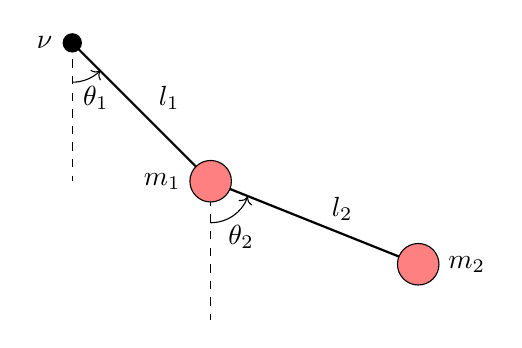
\begin{tikzpicture}

        \coordinate (O) at (0,0);

        \coordinate[yshift=-5pt,xshift=-5pt] (OL) at (O);

        \coordinate[yshift=-50pt] (OE) at (O);

        \coordinate[yshift=-50pt,xshift=50pt] (M1) at (O);

        \coordinate[yshift=-15] (MA) at (M1);

        \coordinate[yshift=-50pt] (ME) at (M1);

        \coordinate[yshift=-30pt,xshift=75pt] (M2) at (M1);

        \coordinate[yshift=-25,xshift=-25] (L) at (O);

        \draw[thick] (O) -- (M1) node[midway,xshift=10pt,yshift=5pt] {$l_1$} -- (M2) node[midway,xshift=10pt,yshift=5pt] {$l_2$};

        \draw[dashed] (O) -- (OE);

        \draw[dashed] (M1) -- (ME);


        \filldraw[color=black,fill=red!50] (M1) circle [radius=7.5pt];
        \filldraw[color=black,fill=red!50] (M2) circle [radius=7.5pt];

        \node[yshift=-20pt,xshift=8.5pt] at (O) {$\theta_1$};

        \node[yshift=-20pt,xshift=11pt] at (M1) {$\theta_2$};

        \node[xshift=-17.5pt] at (M1) {$m_1$};

        \node[xshift=17.5pt] at (M2) {$m_2$};

        %\draw[gray,ultra thick] (-3,0) -- (3,0);

        %\draw[->] (L) -- (OL);

        \node[xshift=-10pt] at (O) {$\nu$};

        % \draw[gray] (-3,0) -- (-2.5,0.35);

        % \draw[gray] (-2.5,0) -- (-2,0.35);

        % \draw[gray] (-2,0) -- (-1.5,0.35);

        % \draw[gray] (-1.5,0) -- (-1,0.35);

        % \draw[gray] (-1,0) -- (-0.5,0.35);

        % \draw[gray] (-0.5,0) -- (0,0.35);

        % \draw[gray] (0,0) -- (0.5,0.35);

        % \draw[gray] (0.5,0) -- (1,0.35);

        % \draw[gray] (1,0) -- (1.5,0.35);

        % \draw[gray] (1.5,0) -- (2,0.35);

        % \draw[gray] (2,0) -- (2.5,0.35);

        % \draw[gray] (2.5,0) -- (3,0.35);

        \fill[black] (O) circle [radius=3.5pt];

        \draw[->] (0,-0.5) arc (-90:-45:0.5);

        \draw[->] (MA) arc (-90:-20:0.5);
    \end{tikzpicture}
    \caption{Schematisk figur över en matematisk dubbelpendel.}
    \label{fig:double_pendulum_schematic}
\end{figure}

% Den enda accelerationen som verkar på massorna $m_1$, $m_2$ antas vara tyngdaccelerationen $g$. 

% vara massorna för respektive enkla pendel, och låt $l_1$, $l_2$ vara längden av respektive pendels snöre/stav. För denna rapport kommer vi bara behandla matematiska pendlar, vilket innebär att massorna $m_1$, $m_2$ antas vara punktformiga och pendels snören anses vara masslösa. 


% Även om det är rent matematiskt möjligt att härleda formlerna som beskriver en dubbelpendels rörelse med klassisk mekanik, anses det

\subsection{Lagrange-mekanik}

För att lösa mer komplexa problem, som exempelvis dubbelpendeln, är det ofta lättare att använda Lagranges ekvationer för att beskriva dess rörelse. Även om det är teoretiskt möjligt att beskriva en dubbelpendels rörelse med klassisk newtonsk mekanik, kan det fort bli mödosamt och därmed används Lagranges ekvationer istället.

En beskrivning av ett system med Lagranges ekvationer består oftast av the Lagrangian $\Lagr$ \cite{book:classical_mechanics:Morin2007}, där $T$ och $V$ är systemets kinetiska respektive lägesenergi, se ekvation (\ref{eq:Lagr}).
\begin{equation} %% todo: varför är det [2] på referensen?
    \Lagr = T - V
    \label{eq:Lagr}
\end{equation}
Sedan ger Euler-Lagrange ekvationen (\ref{eq:euler_lagrange_equation}) att den ekvation som uppfyller (\ref{eq:Lagr}) är den ekvation som beskriver systemets rörelse \cite{book:classical_mechanics:Morin2007}.
\begin{equation}
    \frac{d}{dt}\left( \frac{\partial \Lagr}{\partial \dot{q_{i}}} \right) - \frac{\partial \Lagr}{\partial q_{i}} = 0,
    \label{eq:euler_lagrange_equation}
\end{equation}
för varje $i = 1,2,3,\ldots$. Motivering och härledning av både (\ref{eq:Lagr}) och (\ref{eq:euler_lagrange_equation}) ges i appendix (TODO). %todo

\subsection{Härledning av dubbelpendels rörelseekvationer}

Härledningen utgår från figur \ref{fig:double_pendulum_schematic}, där dubbelpendeln ritats in i ett koordinatsystem där origo utgår från vridpunkten $\nu$. De punktformiga massorna $m_1$ och $m_2$ har koordinaterna $(x_1,y_1)$ respektive $(x_2,y_2)$.

Vi kan beskriva punkterna $x_1$, $x_2$, $y_1$ och $y_2$ går att beskriva genom trigonometri enligt:
\begin{align}
    x_1 & = l_1 \sin{\theta_1} \label{eq:x_1}                      \\
    y_1 & = -l_1\cos{\theta_1} \label{eq:y_1}                      \\
    x_2 & = l_1\sin{\theta_1} + l_2\sin{\theta_2} \label{eq:x_2}   \\
    y_2 & = -l_1\cos{\theta_1} - l_2\cos{\theta_2}. \label{eq:y_2}
\end{align}

Eftersom tidsderivatan av sträcka/position är hastighet, kan vi få hastigheterna $\dot{x}_1$, $\dot{y}_1$, $\dot{x}_2$ och $\dot{y}_2$ enligt:
\begin{align}
    \dot{x}_1 & = \dot{\theta}_1 l_1 \cos{\theta_1} \label{eq:x_1:dot}                   \\
    \dot{y}_1 & = \dot{\theta}_1 l_1 \sin{\theta_1} \label{eq:y_1:dot}                   \\
    \dot{x}_2 & = \dot{\theta}_1 l_1 \cos{\theta_1} + \dot{\theta}_2 l_2 \cos{\theta_2} \label{eq:x_2:dot}  \\
    \dot{y}_2 & = \dot{\theta}_1 l_1 \sin{\theta_1} + \dot{\theta}_2 l_2 \sin{\theta_2}. \label{eq:y_2:dot}
\end{align}

Vi kan därmed definiera dubbelpendelns potentiella energi $V$ som summan av den potentiella energin för respektive massa. Detta ger:
\begin{align}
    V                                              & = m_1gy_1 + m_2gy_2 \notag                                                       \\
    (\ref{eq:y_1}),\/ (\ref{eq:y_2}) \Rightarrow V & = -(m_1 + m_2)gl_1\cos{\theta_1} - m_2gl_2\cos{\theta_2}. \label{eq:V/potential_energy}
\end{align}

Vi kan också bestämma dubbelpendelns kinetiska energi $T$ enligt:
\begin{align}
    T   &= \frac{1}{2} m_1 v_{1}^{2} + \frac{1}{2}m_2v_2^2 \notag \\
        &= \frac{1}{2}m_1\left(\dot{x}_1^2 + \dot{y}_1^2\right) + \frac{1}{2}m_2\left(\dot{x}_2^2 + \dot{y}_2^2\right) \notag \\ %% TODO; motivera kanske varför v^2 = v_x^2 + v_y^2
    (\ref{eq:x_1:dot}) - (\ref{eq:y_2:dot}) \Rightarrow &= \frac{1}{2}m_1\left(\dot{\theta}_1^2 l_1^2 \cos^2{\theta_1} + \dot{\theta}_1^2 l_1^2 \sin^2{\theta_1}\right) + \frac{1}{2}m_2
    \left(
        \dot{\theta}_1^2 l_1^2 \cos^2{\theta_1}\right. \notag \\
        &\quad + 2\dot{\theta}_1\dot{\theta}_2l_1l_2\cos{\theta_1}\cos{\theta_2}
        + \dot{\theta}_2^2l_2^2\cos^2{\theta_2} \dot{\theta}_1^2l_1^2\sin^2{\theta_1} \notag \\
        &\quad + \left.2\dot{\theta}_1\dot{\theta}_2l_1l_2\sin{\theta_1}\sin{\theta_2} + \dot{\theta}_2^2l_2^2\sin^2{\theta_2}
    \right) \notag \\
    \Rightarrow &= \frac{1}{2}m_1\dot{\theta}_1^2l_1^2\left(\cos^2{\theta_1} + \sin^2{\theta_1}\right) + \frac{1}{2}m_2\left( \dot{\theta}_1^2l_1^2\left(\sin^2{\theta_1} + \cos^2{\theta_1}\right) \right. \notag \\
    &\quad + \left.\dot{\theta}_2^2l_2^2\left(\sin^2{\theta_2} + \cos^2{\theta_2}\right) 2\dot{\theta}_1\dot{\theta}_2l_1l_2\left(\cos{\theta_1}\cos{\theta_2} + \sin{\theta_1}\sin{\theta_2}\right)\right). \notag
\end{align}

Eftersom $\sin^2{\theta} + \cos^2{\theta} = 1$ och $\cos(\theta_1 - \theta_2) = \cos{\theta_1}\cos{\theta_2} + \sin{\theta_1}\sin{\theta_2}$ (trigonometriska ettan respektive subtraktionsformeln för cosinus) kan vi förenkla uttrycket till:

\begin{equation}
    T = \frac{1}{2}m_1\dot{\theta}_1^2l_1^2 + \frac{1}{2}m_2\left(\dot{\theta}_1^2l_1^2 + \dot{\theta}_2^2l_2 + 2\dot{\theta}_1\dot{\theta}_2l_1l_2\cos(\theta_1-\theta_2)\right). \label{eq:T/kinetic_energy_simplified}
\end{equation}

Nu när vi har uttryckt $V$ och $T$ som funktioner av $\theta_1$ och $\theta_2$, kan vi beräkna $\Lagr$. Enligt (\ref{eq:Lagr}), (\ref{eq:V/potential_energy}) och (\ref{eq:T/kinetic_energy_simplified}) får vi att:
\begin{align}
    \Lagr               &= T - V \notag \\
                        &= \frac{1}{2}m_1\dot{\theta}_1^2l_1^2 + \frac{1}{2}m_2\left(\dot{\theta}_1^2l_1^2 + \dot{\theta}_2^2l_2^2 + 2\dot{\theta}_1\dot{\theta}_2l_1l_2\cos(\theta_1-\theta_2)\right) \notag \\
                        &\quad - \left(-(m_1 + m_2)gl_1\cos{\theta_1} - m_2gl_2\cos{\theta_2}\right) \notag \\
    \Rightarrow \Lagr   &= \frac{1}{2}m_1\dot{\theta}_1^2l_1^2 + \frac{1}{2}m_2\left(\dot{\theta}_1^2l_1^2 + \dot                {\theta}_2^2l_2^2 + 2\dot{\theta}_1\dot{\theta}_2l_1l_2\cos(\theta_1-\theta_2)\right) \notag \\
                        &\quad + (m_1 + m_2)gl_1\cos{\theta_1} + m_2gl_2\cos{\theta_2} \label{eq:Lagr_simplified}
\end{align}

\subsubsection{Tillämpning av Euler-Lagrange ekvationen}

Vi ska nu använda ekvation (\ref{eq:Lagr_simplified}) i Euler-Lagrange ekvationen (\ref{eq:euler_lagrange_equation}) för att lösa ut ekvationen som beskriver vinklarna $\theta_1$ och $\theta_2$ i dubbelpendeln. Vi beräknar för fallet för $q_i=\theta_1$.

Deriveringsregler för att bestämma $ \frac{\partial \Lagr}{\partial \dot{\theta}_1}$ och $\frac{d}{dt}\!\left(\frac{\partial \Lagr}{\partial \dot{\theta}_1}\right)$ ger:
\begin{align}
    \frac{\partial \Lagr}{\partial \dot{\theta}_1} &= m_1l_1^2\dot{\theta}_1+ m_2l_1^2\dot{\theta}_1 + m_2l_1l_2\dot{\theta}_2\cos(\theta_1-\theta_2) \notag \\
    \Rightarrow \frac{d}{dt}\left(\frac{\partial \Lagr}{\partial \dot{\theta}_1}\right) &= m_1l_1^2\ddot{\theta}_1 + m_2l_1^2\ddot{\theta}_1 + m_2l_1l_2\ddot{\theta}_2\cos(\theta_1-\theta_2) \notag\\
    &\quad - m_2l_1l_2\dot{\theta}_2\sin(\theta_1-\theta_2)(\dot{\theta}_1-\dot{\theta}_2) \notag \\
    \Rightarrow \frac{d}{dt}\left(\frac{\partial \Lagr}{\partial \dot{\theta}_1}\right) &= \left(m_1+m_2\right)l_1^2\ddot{\theta}_1 + m_2l_1l_2\ddot{\theta}_2\cos(\theta_1-\theta_2) \notag \\
    &\quad - m_2l_1l_2\dot{\theta}_1\dot{\theta}_2\sin(\theta_1-\theta_2) + m_2l_1l_2\dot{\theta}_2^2\sin(\theta_1-\theta_2).
\end{align}

Deriveringsregler för att bestämma $\frac{\partial \Lagr}{\partial \theta_1}$ ger:
\begin{align}
    \frac{\partial \Lagr}{\partial \theta_1} &= -m_2l_1l_2\dot{\theta}_1\dot{\theta}_2\sin(\theta_1-\theta_2) - \left(m_1 + m_2\right)gl_1\sin{\theta_1}.
\end{align}

Insättning av detta i (\ref{eq:euler_lagrange_equation}) ger:
\begin{align}
    0 &=\left(m_1+m_2\right)l_1^2\ddot{\theta}_1 + m_2l_1l_2\ddot{\theta}_2\cos(\theta_1-\theta_2)
    - m_2l_1l_2\dot{\theta}_1\dot{\theta}_2\sin(\theta_1-\theta_2) \notag \\
    &\quad + m_2l_1l_2\dot{\theta}_2^2\sin(\theta_1-\theta_2) + m_2l_1l_2\dot{\theta}_1\dot{\theta}_2\sin(\theta_1-\theta_2) + \left(m_1 + m_2\right)gl_1\sin{\theta_1} \notag\\
    \Leftrightarrow 0 &= \left(m_1+m_2\right)l_1\ddot{\theta}_1 + m_2l_2\ddot{\theta}_2\cos(\theta_1-\theta_2)
    + m_2l_2\dot{\theta}_2^2\sin(\theta_1-\theta_2) \notag \\
    &\quad + \left(m_1 + m_2\right)g\sin{\theta_1}. \label{eq:theta_1_solution}
\end{align}

Därmed är (\ref{eq:theta_1_solution}) ekvationen som beskriver vinkeln $\theta_1$ i dubbelpendeln.
\chapter*{Teoretisk genomgång}
\refstepcounter{chapter}

\section{Kaosteori}

Kaosteori är ett tvärvetenskapligt forskningsområde område som fokuserar på att studera mönster hos deterministiska system som är extremt känsliga till begynnelsevillkor \cite{britannica_chaos_theory_2025}. Med detta menas att, om inte exakt samma 

\section{Lagrange-mekanik}

För att lösa mer komplexa problem, som exempelvis dubbelpendeln, är det oftare lättare att använda Lagrange-mekanik för att beskriva dess rörelse. Även om det är teoretiskt sätt möjligt att beskriva en dubbelpendels rörelse med klassisk newtonsk mekanik, kan det fort bli mödosamt och onödigt krångligt. Lagrange-mekanik är egentligen bara en annan matematisk metod för att beskriva omvärlden, vilket i en viss typ av problem, blir betydligt lättare att lösa.

%För att lösa mer komplexa problem, som exempelvis dubbelpendeln, är det ofta lättare att använda Lagranges ekvationer för att beskriva dess rörelse. Även om det är teoretiskt möjligt att beskriva en dubbelpendels rörelse med klassisk newtonsk mekanik, kan det fort bli mödosamt och därmed används Lagranges ekvationer istället.

% En beskrivning av ett system med Lagranges ekvationer består oftast av the Lagrangian $\Lagr$ \cite{book:classical_mechanics:Morin2007}, där $T$ och $V$ är systemets kinetiska respektive lägesenergi, se ekvation (\ref{eq:Lagr}).
% \begin{equation} %% todo: varför är det [2] på referensen?
%     \Lagr = T - V
%     \label{eq:Lagr}
% \end{equation}
% Sedan ger Euler-Lagrange ekvationen (\ref{eq:euler_lagrange_equation}) att den ekvation som uppfyller (\ref{eq:Lagr}) är den ekvation som beskriver systemets rörelse \cite{book:classical_mechanics:Morin2007}.
% \begin{equation}
%     \frac{d}{dt}\left( \frac{\partial \Lagr}{\partial \dot{q_{i}}} \right) - \frac{\partial \Lagr}{\partial q_{i}} = 0,
%     \label{eq:euler_lagrange_equation}
% \end{equation}
% för varje $i = 1,2,3,\ldots$.

\subsection{Principen om minsta verkan}

Lagrange-mekanik bygger sin grund på \emph{principen om minsta verkan}, eller ibland även kallad \emph{principen om stationär verkan} \cite{Manton2013PrincipleLeastAction}. Denna princip säger därmed att ett objekt kommer alltid att sträva efter att färdas den väg som minimerar den fysikaliska \emph{verkan} \cite[s.2]{Manton2013PrincipleLeastAction}. Detta är så fysikaliskt grundläggande, att nästan all fysik kan härledas ur detta grundläggande antagande \cite{Manton2013PrincipleLeastAction}. Givet att vi har ett objekt $Q$ som rör sig längs $x(t)$, där $Q$ har startpunkten $x(t_1)$ och slutpunkten $x(t_2)$, samt att $T(t)$ och $V(t)$ är objektets rörelse respektive kinetiska energi, definieras verkan $S$ inom tidsintervallet $t_1\leq t \leq t_2$ som \cite[s.10]{Manton2013PrincipleLeastAction}:
\begin{equation} 
    S = \int_{t_1}^{t_2}\left(T(t)-V(t)\right)dt. \label{eq:action_definition}
\end{equation} 
Denna storhet har enheten [Js] och har dimensionerna (Energi $\times$ Tid) \cite[s.221]{book:classical_mechanics:Morin2007}. Själva differensen $T(t) - V(t)$ visar sig vara så relevant inom fysiken, att den har fått namnet 'the Lagrangian' och brukar betecknas $\Lagr$ \cite[s.218]{book:classical_mechanics:Morin2007}, det vill säga
\footnote{Varför $\Lagr = T(t) - V(t)$ är så viktigt i (\ref{eq:action_definition}) kan tyckas konstigt. Varför ska \emph{differensen} av kinetiska och potentiella energin spela någon roll? }:
\begin{equation} %% todo: varför är det [2] på referensen?
    \Lagr = T - V
    \label{eq:Lagr}
\end{equation}
Principen om minsta verkan säger att fysikens lagar strävar efter att förminska (\ref{eq:action_definition})\footnote{Egentligen, rent matematiskt, strävar verkan $S$ att hitta ett stationärt värde av $S$, det vill säga en lokal extrem- eller terrasspunkt till grafen av $S$. Detta är anledningen varför principen även kallas för \emph{principen om stationär verkan} \cite[s.222]{book:classical_mechanics:Morin2007}.}.

För att bestämma ett objekts väg som minimerar verkan $S$ används \emph{Euler-Lagrange ekvationen} \cite[s. 222]{book:classical_mechanics:Morin2007} se ekvation (\ref{eq:euler_lagrange_equation}). I ekvation (\ref{eq:euler_lagrange_equation}) är $i = 1,2,3,\ldots$, och normalt sätt betecknar de olika koordinataxlarna i systemet. Härledning av (\ref{eq:euler_lagrange_equation}) ges i appendix A. %% TODO, härledning av euler-lagrange ekvationen
\begin{equation}
    \frac{d}{dt}\left( \frac{\partial \Lagr}{\partial \dot{q_{i}}} \right) - \frac{\partial \Lagr}{\partial q_{i}} = 0,
    \label{eq:euler_lagrange_equation}
\end{equation}

%\subsubsection{Pedagogiskt exempel på tillämpning av Lagrange-mekanik}
%För att ge ett exempel på hur ekvation (\ref{eq:euler_lagrange_equation}) kan användas rent fysikaliskt\footnote{Hos många studenter kan det till en början kännas 'udda' varför (\ref{eq:Lagr}) och (\ref{eq:euler_lagrange_equation}) ens är relevanta. Därför tas detta exempel med, för att ge en viss intuition till att (\ref{eq:euler_lagrange_equation}) funkar.}, tas ett exempel på en boll med massan $m$. Om vi släpper bollen från vila, och låter den falla fritt (utan något luftmotstånd), kommer den ha fallit höjden $h$ under 1 sekund. Vi vet enligt de välkända kinematiska formlerna \cite{formelsamling} att $h=\frac{gt^2}{2}$, dvs bollen kommer att ha färdats $\frac{g}{2}$ m efter 1 sekund.  

% Verkan är en fysikalisk storhet som beskriver summan av , där om vi har ett objekt som rör sig mellan två punkter $x(t_1)$ och $x(t_2)$ inom tidsintervallet $(t_2 - t_1)$, så definieras verkan $S$ som \cite[s.10]{Manton2013PrincipleLeastAction}:
% \begin{equation} 
%     S = \int_{t_1}^{t_2}\left(T(t)-V(t)\right)dt. \label{eq:action_definition}
% \end{equation} 



% Det kan kännas spontant udda varför ekvationerna (\ref{eq:Lagr}) och (\ref{eq:euler_lagrange_equation}) ens är relevanta. Dessa ekvationer är dock en konsekvens av \emph{principen om minsta verkan}, vilket säger att ett objekt kommer alltid sträva efter att färdas den väg som minimerar den fysikaliska verkan \cite[s.2]{Manton2013PrincipleLeastAction}. Verkan är en fysikalisk storhet, där om vi har ett objekt som rör sig mellan två punkter $x(t_1)$ och $x(t_2)$ inom tidsintervallet $(t_2 - t_1)$, så definieras verkan $S$ som \cite[s.10]{Manton2013PrincipleLeastAction}:
% \begin{equation} 
%     S = \int_{t_1}^{t_2}\left(T(t)-V(t)\right)dt. \label{eq:action_definition}
% \end{equation} 
% Denna storhet har enheten [Js] och har dimensionerna (Energi $\times$ Tid). Det visar sig att \emph{principen om minsta verkan} är en princip som är minst lika fundamental som t.ex energiprincipen,


%Motivering och härledning av både (\ref{eq:Lagr}) och (\ref{eq:euler_lagrange_equation}) ges i appendix (TODO). %todo



\section{Dubbelpendeln}
Om två vanliga enkla pendlar är sammankopplade sägs de bilda en dubbelpendel, se figur \ref{fig:double_pendulum_schematic}. Den första pendeln består av en punktformig massa $m_1$ som är kopplad till en masslös pinne med längden $l_1$, vilket sitter i en friktionslös rotationspunkt $\nu$. Den andra pendeln består också av en punktformig massa $m_2$ som är kopplad till en masslös pinne med längden $l_2$. Denna andra pendeln har sin friktionslösa rotationspunkt tillkopplad i $m_1$. Den enda kraften som verkar på respektive massa är tyngdkraften.

Låt vinklarna $\theta_1$, $\theta_2$ vara vinklarna mellan den lodräta linjen från rotationspunkten och den faktiska positionen av pendeln, se figur \ref{fig:double_pendulum_schematic}. Vinklarna $\theta_1$ och $\theta_2$ är inte begränsade mellan $-\pi \leq \theta_{1,2} \leq \pi$, dvs de kan rotera fritt hur många varv som helst runt rotationspunkterna. Detta innebär självklart att respektive pendel inte kommer påverkas av varandra, t.ex att de inte kan slå in i varandra.

\begin{figure}[h!]
    \centering
    %\includegraphics[scale=1]{Double-pendulum-system.png}
    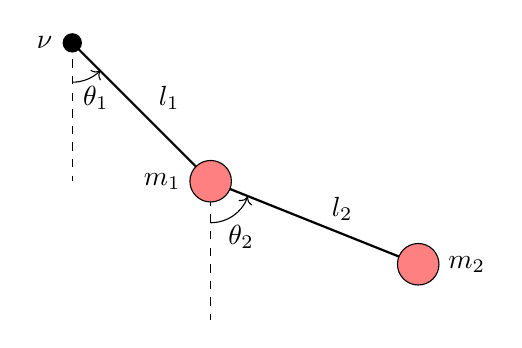
\begin{tikzpicture}

        \coordinate (O) at (0,0);

        \coordinate[yshift=-5pt,xshift=-5pt] (OL) at (O);

        \coordinate[yshift=-50pt] (OE) at (O);

        \coordinate[yshift=-50pt,xshift=50pt] (M1) at (O);

        \coordinate[yshift=-15] (MA) at (M1);

        \coordinate[yshift=-50pt] (ME) at (M1);

        \coordinate[yshift=-30pt,xshift=75pt] (M2) at (M1);

        \coordinate[yshift=-25,xshift=-25] (L) at (O);

        \draw[thick] (O) -- (M1) node[midway,xshift=10pt,yshift=5pt] {$l_1$} -- (M2) node[midway,xshift=10pt,yshift=5pt] {$l_2$};

        \draw[dashed] (O) -- (OE);

        \draw[dashed] (M1) -- (ME);


        \filldraw[color=black,fill=red!50] (M1) circle [radius=7.5pt];
        \filldraw[color=black,fill=red!50] (M2) circle [radius=7.5pt];

        \node[yshift=-20pt,xshift=8.5pt] at (O) {$\theta_1$};

        \node[yshift=-20pt,xshift=11pt] at (M1) {$\theta_2$};

        \node[xshift=-17.5pt] at (M1) {$m_1$};

        \node[xshift=17.5pt] at (M2) {$m_2$};

        %\draw[gray,ultra thick] (-3,0) -- (3,0);

        %\draw[->] (L) -- (OL);

        \node[xshift=-10pt] at (O) {$\nu$};

        % \draw[gray] (-3,0) -- (-2.5,0.35);

        % \draw[gray] (-2.5,0) -- (-2,0.35);

        % \draw[gray] (-2,0) -- (-1.5,0.35);

        % \draw[gray] (-1.5,0) -- (-1,0.35);

        % \draw[gray] (-1,0) -- (-0.5,0.35);

        % \draw[gray] (-0.5,0) -- (0,0.35);

        % \draw[gray] (0,0) -- (0.5,0.35);

        % \draw[gray] (0.5,0) -- (1,0.35);

        % \draw[gray] (1,0) -- (1.5,0.35);

        % \draw[gray] (1.5,0) -- (2,0.35);

        % \draw[gray] (2,0) -- (2.5,0.35);

        % \draw[gray] (2.5,0) -- (3,0.35);

        \fill[black] (O) circle [radius=3.5pt];

        \draw[->] (0,-0.5) arc (-90:-45:0.5);

        \draw[->] (MA) arc (-90:-20:0.5);
    \end{tikzpicture}
    \caption{Schematisk figur över en matematisk dubbelpendel.}
    \label{fig:double_pendulum_schematic}
\end{figure}


% Den första pendeln består av en masslös pinne med längden $l_1$ som sitter i en friktionslös vridpunkt $\nu$. Vid änden av pinnen sitter även en punktformig massa $m_1$. Därefter kopplas en till masslös pinne med längden $l_2$ på $m_1$ så att pinnen kan rotera friktionsfritt. Dessutom finns en till punktformig massa $m_2$ tillkopplad på änden av pinnen med längden $l_2$. Eftersom pinnarna är masslösa och all friktion kan försummas, kan denna uppställning av en dubbelpendel beskrivas som en matematisk dubbelpendel. Låt vinklarna $\theta_1$, $\theta_2$ vara vinklarna normalen taket och pinnarna till för respektive enkel pendel. Den resulterande accelerationen på massorna $m_1$, $m_2$ är tyngdaccelerationen $g$.

% Eftersom pinnarna är masslösa, massorna $m_1$, $m_2$ är punktformiga och all friktion försummas, sägs dubbelpendeln vara matematisk. Därmed kommer energin i hela system bevaras. 

% Den enda accelerationen som verkar på massorna $m_1$, $m_2$ antas vara tyngdaccelerationen $g$. 

% vara massorna för respektive enkla pendel, och låt $l_1$, $l_2$ vara längden av respektive pendels snöre/stav. För denna rapport kommer vi bara behandla matematiska pendlar, vilket innebär att massorna $m_1$, $m_2$ antas vara punktformiga och pendels snören anses vara masslösa. 


% Även om det är rent matematiskt möjligt att härleda formlerna som beskriver en dubbelpendels rörelse med klassisk mekanik, anses det



\subsection{Härledning av dubbelpendels rörelseekvationer} \label{sec:härledning_av_dubbelpendeln}

Härledningen utgår från figur \ref{fig:double_pendulum_schematic}, där dubbelpendeln ritats in i ett koordinatsystem där origo utgår från vridpunkten $\nu$. De punktformiga massorna $m_1$ och $m_2$ har koordinaterna $(x_1,y_1)$ respektive $(x_2,y_2)$.

Vi kan beskriva punkterna $x_1$, $x_2$, $y_1$ och $y_2$ genom trigonometri enligt:
\begin{align}
    x_1 & = l_1 \sin{\theta_1} \label{eq:x_1}                      \\
    y_1 & = -l_1\cos{\theta_1} \label{eq:y_1}                      \\
    x_2 & = l_1\sin{\theta_1} + l_2\sin{\theta_2} \label{eq:x_2}   \\
    y_2 & = -l_1\cos{\theta_1} - l_2\cos{\theta_2}. \label{eq:y_2}
\end{align}

Eftersom tidsderivatan av sträcka/position är hastighet, kan vi få hastigheterna $\dot{x}_1$, $\dot{y}_1$, $\dot{x}_2$ och $\dot{y}_2$ enligt:
\begin{align}
    \dot{x}_1 & = \dot{\theta}_1 l_1 \cos{\theta_1} \label{eq:x_1:dot}                   \\
    \dot{y}_1 & = \dot{\theta}_1 l_1 \sin{\theta_1} \label{eq:y_1:dot}                   \\
    \dot{x}_2 & = \dot{\theta}_1 l_1 \cos{\theta_1} + \dot{\theta}_2 l_2 \cos{\theta_2} \label{eq:x_2:dot}  \\
    \dot{y}_2 & = \dot{\theta}_1 l_1 \sin{\theta_1} + \dot{\theta}_2 l_2 \sin{\theta_2}. \label{eq:y_2:dot}
\end{align}

Vi kan därmed definiera dubbelpendelns potentiella energi $V$ som summan av den potentiella energin för respektive massa. Detta ger:
\begin{align}
    V                                              & = m_1gy_1 + m_2gy_2 \notag                                                       \\
    (\ref{eq:y_1}),\/ (\ref{eq:y_2}) \Rightarrow V & = -(m_1 + m_2)gl_1\cos{\theta_1} - m_2gl_2\cos{\theta_2}. \label{eq:V/potential_energy}
\end{align}

Vi kan också bestämma dubbelpendelns kinetiska energi $T$ enligt:
\begin{align}
    T   &= \frac{1}{2} m_1 v_{1}^{2} + \frac{1}{2}m_2v_2^2 \notag \\
        &= \frac{1}{2}m_1\left(\dot{x}_1^2 + \dot{y}_1^2\right) + \frac{1}{2}m_2\left(\dot{x}_2^2 + \dot{y}_2^2\right) \notag \\ %% TODO; motivera kanske varför v^2 = v_x^2 + v_y^2
    (\ref{eq:x_1:dot}) - (\ref{eq:y_2:dot}) \Rightarrow &= \frac{1}{2}m_1\left(\dot{\theta}_1^2 l_1^2 \cos^2{\theta_1} + \dot{\theta}_1^2 l_1^2 \sin^2{\theta_1}\right) + \frac{1}{2}m_2
    \left(
        \dot{\theta}_1^2 l_1^2 \cos^2{\theta_1}\right. \notag \\
        &\quad + 2\dot{\theta}_1\dot{\theta}_2l_1l_2\cos{\theta_1}\cos{\theta_2}
        + \dot{\theta}_2^2l_2^2\cos^2{\theta_2} \dot{\theta}_1^2l_1^2\sin^2{\theta_1} \notag \\
        &\quad + \left.2\dot{\theta}_1\dot{\theta}_2l_1l_2\sin{\theta_1}\sin{\theta_2} + \dot{\theta}_2^2l_2^2\sin^2{\theta_2}
    \right) \notag \\
    \Rightarrow &= \frac{1}{2}m_1\dot{\theta}_1^2l_1^2\left(\cos^2{\theta_1} + \sin^2{\theta_1}\right) + \frac{1}{2}m_2\left( \dot{\theta}_1^2l_1^2\left(\sin^2{\theta_1} + \cos^2{\theta_1}\right) \right. \notag \\
    &\quad + \left.\dot{\theta}_2^2l_2^2\left(\sin^2{\theta_2} + \cos^2{\theta_2}\right) 2\dot{\theta}_1\dot{\theta}_2l_1l_2\left(\cos{\theta_1}\cos{\theta_2} + \sin{\theta_1}\sin{\theta_2}\right)\right). \notag
\end{align}

Eftersom $\sin^2{\theta} + \cos^2{\theta} = 1$ och $\cos{\theta_1}\cos{\theta_2} + \sin{\theta_1}\sin{\theta_2} = \cos(\theta_1 - \theta_2)$ (trigonometriska ettan respektive subtraktionsformeln för cosinus) kan vi förenkla uttrycket till:

\begin{equation}
    T = \frac{1}{2}m_1\dot{\theta}_1^2l_1^2 + \frac{1}{2}m_2\left(\dot{\theta}_1^2l_1^2 + \dot{\theta}_2^2l_2 + 2\dot{\theta}_1\dot{\theta}_2l_1l_2\cos(\theta_1-\theta_2)\right). \label{eq:T/kinetic_energy_simplified}
\end{equation}

Nu när vi har uttryckt $V$ och $T$ som funktioner av $\theta_1$ och $\theta_2$, kan vi beräkna $\Lagr$. Enligt (\ref{eq:Lagr}), (\ref{eq:V/potential_energy}) och (\ref{eq:T/kinetic_energy_simplified}) får vi att:
\begin{align}
    \Lagr               &= T - V \notag \\
                        &= \frac{1}{2}m_1\dot{\theta}_1^2l_1^2 + \frac{1}{2}m_2\left(\dot{\theta}_1^2l_1^2 + \dot{\theta}_2^2l_2^2 + 2\dot{\theta}_1\dot{\theta}_2l_1l_2\cos(\theta_1-\theta_2)\right) \notag \\
                        &\quad - \left(-(m_1 + m_2)gl_1\cos{\theta_1} - m_2gl_2\cos{\theta_2}\right) \notag \\
    \Rightarrow \Lagr   &= \frac{1}{2}m_1\dot{\theta}_1^2l_1^2 + \frac{1}{2}m_2\left(\dot{\theta}_1^2l_1^2 + \dot                {\theta}_2^2l_2^2 + 2\dot{\theta}_1\dot{\theta}_2l_1l_2\cos(\theta_1-\theta_2)\right) \notag \\
                        &\quad + (m_1 + m_2)gl_1\cos{\theta_1} + m_2gl_2\cos{\theta_2}. \label{eq:Lagr_simplified}
\end{align}

\subsubsection{Tillämpning av Euler-Lagrange ekvationen}

Vi ska nu använda ekvation (\ref{eq:Lagr_simplified}) i Euler-Lagrange ekvationen (\ref{eq:euler_lagrange_equation}) för att lösa ut ekvationen som beskriver vinklarna $\theta_1$ och $\theta_2$ i dubbelpendeln. Vi beräknar för fallet för $q_i=\theta_1$.

Deriveringsregler för att bestämma $ \frac{\partial \Lagr}{\partial \dot{\theta}_1}$ och $\frac{d}{dt}\!\left(\frac{\partial \Lagr}{\partial \dot{\theta}_1}\right)$ ger:
\begin{align}
    \frac{\partial \Lagr}{\partial \dot{\theta}_1} &= m_1l_1^2\dot{\theta}_1+ m_2l_1^2\dot{\theta}_1 + m_2l_1l_2\dot{\theta}_2\cos(\theta_1-\theta_2) \notag \\
    \Rightarrow \frac{d}{dt}\left(\frac{\partial \Lagr}{\partial \dot{\theta}_1}\right) &= m_1l_1^2\ddot{\theta}_1 + m_2l_1^2\ddot{\theta}_1 + m_2l_1l_2\ddot{\theta}_2\cos(\theta_1-\theta_2) \notag\\
    &\quad - m_2l_1l_2\dot{\theta}_2\sin(\theta_1-\theta_2)(\dot{\theta}_1-\dot{\theta}_2) \notag \\
    \Rightarrow \frac{d}{dt}\left(\frac{\partial \Lagr}{\partial \dot{\theta}_1}\right) &= \left(m_1+m_2\right)l_1^2\ddot{\theta}_1 + m_2l_1l_2\ddot{\theta}_2\cos(\theta_1-\theta_2) \notag \\
    &\quad - m_2l_1l_2\dot{\theta}_1\dot{\theta}_2\sin(\theta_1-\theta_2) + m_2l_1l_2\dot{\theta}_2^2\sin(\theta_1-\theta_2). \label{eq:Lagr_time_derivative:respect_theta_1_dot}
\end{align}

Deriveringsregler för att bestämma $\frac{\partial \Lagr}{\partial \theta_1}$ ger:
\begin{align}
    \frac{\partial \Lagr}{\partial \theta_1} &= -m_2l_1l_2\dot{\theta}_1\dot{\theta}_2\sin(\theta_1-\theta_2) - \left(m_1 + m_2\right)gl_1\sin{\theta_1}. \label{eq:Lagr_derivative:repsect_theta_1}
\end{align}

Insättning av (\ref{eq:Lagr_time_derivative:respect_theta_1_dot}) och (\ref{eq:Lagr_derivative:repsect_theta_1}) i (\ref{eq:euler_lagrange_equation}) ger att:
\begin{align}
    0 &=\left(m_1+m_2\right)l_1^2\ddot{\theta}_1 + m_2l_1l_2\ddot{\theta}_2\cos(\theta_1-\theta_2)
    - m_2l_1l_2\dot{\theta}_1\dot{\theta}_2\sin(\theta_1-\theta_2) \notag \\
    &\quad + m_2l_1l_2\dot{\theta}_2^2\sin(\theta_1-\theta_2) + m_2l_1l_2\dot{\theta}_1\dot{\theta}_2\sin(\theta_1-\theta_2) + \left(m_1 + m_2\right)gl_1\sin{\theta_1} \notag\\
    \Leftrightarrow 0 &= \left(m_1+m_2\right)l_1\ddot{\theta}_1 + m_2l_2\ddot{\theta}_2\cos(\theta_1-\theta_2)
    + m_2l_2\dot{\theta}_2^2\sin(\theta_1-\theta_2) \notag \\
    &\quad + \left(m_1 + m_2\right)g\sin{\theta_1}. \label{eq:theta_1_solution}
\end{align}

Därmed är (\ref{eq:theta_1_solution}) ekvationen som beskriver vinkeln $\theta_1$ i dubbelpendeln. Nu ska vi istället lösa Euler-Lagrange ekvationen (\ref{eq:euler_lagrange_equation}) fast för $q_i = \theta_2$.

Deriveringsregler för att bestämma $ \frac{\partial \Lagr}{\partial \dot{\theta}_2}$ och $\frac{d}{dt}\!\left(\frac{\partial \Lagr}{\partial \dot{\theta}_2}\right)$ ger:
\begin{align}
    \frac{\partial \Lagr}{\partial \dot{\theta}_2} &= m_2l_2^2\dot{\theta}_2 + m_2l_1l_2\dot{\theta}_1\cos(\theta_1 - \theta_2) \notag\\
    \Rightarrow \frac{d}{dt}\left(\frac{\partial \Lagr}{\partial \dot{\theta}_2}\right) &= m_2l_2^2\ddot{\theta}_2 + m_2l_1l_2\left(\ddot{\theta}_1\cos(\theta_1-\theta_2) - \dot{\theta}_1\sin(\theta_1 - \theta_2)(\dot{\theta}_1 - \dot{\theta}_2)\right) \notag \\
    \Rightarrow \frac{d}{dt}\left(\frac{\partial \Lagr}{\partial \dot{\theta}_2}\right) &= m_2l_2^2\ddot{\theta}_2 + m_2l_1l_2\ddot{\theta}_1\cos(\theta_1-\theta_2) - m_2l_1l_2\dot{\theta}_1^2\sin(\theta_1-\theta_2) \notag \\
    &\quad + m_2l_1l_2\dot{\theta}_1\dot{\theta}_2\sin(\theta_1 - \theta_2). \label{eq:Lagr_time_derivative:respect_theta_2_dot}
\end{align}

Deriveringsregler för att bestämma $\frac{\partial \Lagr}{\partial \theta_2}$ ger:
\begin{align}
    \frac{\partial \Lagr}{\partial \theta_2} &= m_2l_1l_2\dot{\theta}_1\dot{\theta}_2\sin(\theta_1-\theta_2) - m_2gl_2\sin{\theta_2}.  \label{eq:Lagr_derivative:repsect_theta_2}
\end{align}

Insättning av (\ref{eq:Lagr_time_derivative:respect_theta_2_dot}) och (\ref{eq:Lagr_derivative:repsect_theta_2}) i (\ref{eq:euler_lagrange_equation}) ger:
\begin{align}
    0 &= m_2l_2^2\ddot{\theta}_2 + m_2l_1l_2\ddot{\theta}_1\cos(\theta_1 - \theta_2) - m_2l_1l_2\dot{\theta}_1^2\sin(\theta_1-\theta_2) \notag \\
    &\quad + m_2l_1l_2\dot{\theta_1}\dot{\theta}_2\sin(\theta_1 - \theta_2) - m_2l_1l_2\dot{\theta}_1\dot{\theta}_2\sin(\theta_1-\theta_2) + m_2gl_2\sin{\theta_2} \notag \\
    \Leftrightarrow 0 &= m_2l_2\ddot{\theta}_2 + m_2l_1\ddot{\theta}_1\cos(\theta_1 - \theta_2) - m_2l_1\dot{\theta}_1^2\sin(\theta_1 - \theta_2) + m_2g\sin{\theta_2}. \label{eq:theta_2_solution}
\end{align}

Detta innebär att (\ref{eq:theta_2_solution}) är den ekvation som beskriver vinkeln $\theta_2$ i dubbelpendeln. Därmed har vi nu funnit våra två ekvationer som enligt Euler-Lagrange ekvationen (\ref{eq:euler_lagrange_equation}) beskriver dubbelpendelns rörelse, se ekvationssystemet (\ref{eq:equations_of_motion}):
\begin{equation} \begin{cases}
        0 &= \left(m_1+m_2\right)l_1\ddot{\theta}_1 + m_2l_2\ddot{\theta}_2\cos(\theta_1-\theta_2)
        + m_2l_2\dot{\theta}_2^2\sin(\theta_1-\theta_2) \\
        &\quad + \left(m_1 + m_2\right)g\sin{\theta_1}. \\
        0 &= m_2l_2\ddot{\theta}_2 + m_2l_1\ddot{\theta}_1\cos(\theta_1 - \theta_2) - m_2l_1\dot{\theta}_1^2\sin(\theta_1 - \theta_2) + m_2g\sin{\theta_2}. \label{eq:equations_of_motion}
\end{cases} \end{equation}

Ekvationssystemet i (\ref{eq:equations_of_motion}) går inte att lösa analytiskt, utan måste skrivas om för att få (\ref{eq:equations_of_motion}) till en ordinär första ordningens differentialekvation (ODE). Detta kan göras genom att införa nya beteckningar för vinkelhastigheterna $\omega_1$ och $\omega_2$, dvs $\omega_1 = \dot{\theta_1}$ och $\omega_2 = \dot{\theta_2}$. Därmed kan (\ref{eq:equations_of_motion}) skrivas om enligt ekvationssystemet (\ref{eq:equations_of_motion_with_omega}). 

\begin{equation}
    \begin{cases}
        \dot{\theta}_1 = \omega_1  \\
        \dot{\theta}_2 = \omega_2 \\
        \dot{\omega}_1 = - \frac{m_2l_2\dot{\omega}_2^2\cos(\theta_1 - \theta_2) + m_1l_2\omega_2^2\sin(\theta_1-\theta_2) + (m_1+m_2)g\sin{\theta_1}}{(m_1+m_2)l_1} \\
        \dot{\omega}_2 = - \frac{m_2l_1\dot{\omega}_1\cos(\theta_1-\theta_2) - m_2l_1\omega^2_1\sin(\theta_1 - \theta_2 + m_2g\sin{\theta_2})}{m_2l_2} \label{eq:equations_of_motion_with_omega}
    \end{cases}
\end{equation}

Däremot har (\ref{eq:equations_of_motion_with_omega}) problemet att de tredje och fjärde ekvationerna är sammankopplade (på engelska, 'coupled'). Dessa två måste separeras för att kunna lösas numeriskt.  

\section{Numerisk metod för att lösa differentialekvationer}

Differentialekvationerna i (\ref{eq:equations_of_motion}) är icke-linjära och av andra ordningen, vilket gör de omöjligt att lösa rent analystiskt. Därmed måste ekvationerna lösas numeriskt, vilket kan göras med \emph{Runge-Kuttametoden}. Denna metod\footnote{Egentligen är Runge-Kuttametoden är en familj av metoder, då den innefattar ett flertal metoder, bland annat Eulers stegmetod. Däremot brukas RK4-metoden menas med ''Runge-Kuttametoden'', vilket är den vi kommer att använda här. För vidare förklaring, se \cite{Runge-Kutta_method/Butcher2008}. }, utvecklat och namngivet av de tyska matematikerna Carl Runge och Martin Willhelm Kutta, är en kraftfull metod för att lösa ordinära differentialekvationer (ODE:s) \cite[s. 93]{Runge-Kutta_method/Butcher2008}. 

Runge-Kuttametoden ger oss en metod att lösa ekvationer på formen $x' = f(t,x)$, där $x(t)$ är den okända funktionen. Metoden bygger på att approximera lösningen stegvis med ett litet $h$, men istället för att bara beräkna nuvarande lutningen (det som sker i Eulers metod), så beräknas flera mellanliggande lutningar där ett viktad medelvärde istället dras. 


\subsection{Behandling av dubbelpendelns rörelseekvationer för att möjliggöra RK4-metoden}


\subsection{Allmänna definitionen av RK4-metoden}

Låt $\mathbf{x}$ vara en tillståndsvektor sådan att $\mathbf{x} = [x_1, x_2, \ldots, x_n]^T$, $\mathbf{x}' = \frac{d\mathbf{x}}{dt}$ och låt $\mathbf{f} = [f_1, f_2, \ldots, f_n]^T$. Dessutom har vi begynnelsevärdet TODO Vi vill beräkna värdet av tillståndsvektorn $\bf{x}$ över tidsintervallet $[t_0, t]$ med steglängden $h$. Givet att $\bf{x'} = f(t,x)$, så definieras nästa tillståndsvektor $\bf{x_{n+1}}$ enligt: 
\begin{equation}
    \mathbf{x}_{n+1} = x_n + \frac{h}{6}\left(\mathbf{K}_{1n} + 2\mathbf{K}_{2n} + 2\mathbf{K}_{3n} + \mathbf{K}_{4n}\right),
\end{equation}
\begin{equation}
    t_{n+1} = t_n + h,
\end{equation}
där värdena av $\mathbf{K}_{1n}, \mathbf{K}_{2n}, \mathbf{K}_{3n}$ och $\mathbf{K}_{4n}$ är definierade sådan att:
\begin{align}
    \mathbf{K}_{1n} &= \mathbf{f}(t,\mathbf{x}_n) \\
    \mathbf{K}_{2n} &= \mathbf{f}\left(t + \frac{h}{2}, \mathbf{x}_n + \frac{h}{2}\mathbf{K}_{1n}\right) \\
    \mathbf{K}_{3n} &= \mathbf{f}\left(t + \frac{h}{2}, \mathbf{x}_n + \frac{h}{2}\mathbf{K}_{2n}\right) \\
    \mathbf{K}_{4n} &= \mathbf{f}\left(t + h, \mathbf{x}_n + h\mathbf{K}_{3n}\right)
\end{align}


\footnote{Definitionen av RK4-metoden är hämtat från \cite{Allard2015DoublePendulum/Runge-Kutta-definition}}
\chapter*{Numerisk simulering och metod}
\refstepcounter{chapter}

\section{Behandling av rörelseekvationerna inför simulering}
Som vi visade i sektion \ref{sec:härledning_av_dubbelpendeln}, ekvation (\ref{eq:equations_of_motion}), har vi härlett rörelseekvationerna för dubbelpendeln med hjälp av Lagrange-mekanik. Dessa är:
\begin{equation} \begin{cases}
        0 &= \left(m_1+m_2\right)l_1\ddot{\theta}_1 + m_2l_2\ddot{\theta}_2\cos(\theta_1-\theta_2)
        + m_2l_2\dot{\theta}_2^2\sin(\theta_1-\theta_2) \\
        &\quad + \left(m_1 + m_2\right)g\sin{\theta_1}. \\
        0 &= m_2l_2\ddot{\theta}_2 + m_2l_1\ddot{\theta}_1\cos(\theta_1 - \theta_2) - m_2l_1\dot{\theta}_1^2\sin(\theta_1 - \theta_2) + m_2g\sin{\theta_2}. \label{eq:equations_of_motion_numerical_section}
\end{cases} \end{equation}
För att däremot kunna använda (\ref{eq:equations_of_motion_numerical_section}) med Runge-Kuttametoden, måste de skrivas om till ordinära differentialekvationer på formen $x' = f(x,t)$. Vi börjar med att genomföra substitutionen $\dot{\theta}_1 = \omega_1$ och $\dot{\theta}_2$, vilket ger:
\begin{equation}
    \begin{cases}
        \dot{\theta}_1 &= \omega_1  \\
        \dot{\theta}_2 &= \omega_2 \\
        0 &= (m_1+m_2)l_1\dot{\omega}_1 + m_2l_2\dot{\omega}_2\cos(\theta_1 - \theta_2) + m_2l_2\omega_2^2\sin(\theta_1 - \theta_2) \\
        &\quad + (m_1+m_2)g\sin{\theta_1} \\
        0 &= m_2l_2\dot{\omega}_2 + m_2l_1\dot{\omega}_1\cos(\theta_1 - \theta_2) - m_2l_1\omega_1^2\sin(\theta_1-\theta_2) + m_2g\sin{\theta_2}. \label{eq:equations_of_motion_with_omega_numerical_section}
    \end{cases}
\end{equation}
Däremot är fortfarande tredje och fjärde ekvationerna i (\ref{eq:equations_of_motion_with_omega_numerical_section}) sammankopplade (på engelska, 'coupled'). För att kunna använda (\ref{eq:equations_of_motion_with_omega_numerical_section}) i Runge-kuttametoden gör vi följande substitution enligt (\ref{eq:greek_substitutions}). 
\begin{equation}
    \begin{cases}
        \Delta\theta &= \theta_1 - \theta_2 \\
        \alpha &= (m_1+m_2)l_1 \\
        \beta &= m_2l_2\cos(\Delta\theta) \\
        \gamma &= m_2l_1\cos(\Delta\theta) \\
        \delta &= m_2l_2 \\
        \epsilon &= -m_2l_2\omega_2^2\sin(\Delta\theta) - (m_1 + m_2)g\sin{\theta_1} \\
        \zeta &= m_2l_2\omega_1^2\sin(\Delta\theta) - m_2g\sin{\theta_2}
    \end{cases} \label{eq:greek_substitutions}
\end{equation}
Vi kan nu skriva om ekvationssystemet (\ref{eq:equations_of_motion_with_omega_numerical_section}) med hjälp av substitutionerna i (\ref{eq:greek_substitutions}) enligt:
\begin{equation}
    \begin{cases}
        \dot{\theta}_1 &= \omega_1  \\
        \dot{\theta}_2 &= \omega_2 \\
        0 &= \alpha\dot{\omega}_1 + \beta \dot{\omega}_2 - \epsilon \\
        0 &= \delta\dot{\omega}_2 + \gamma\dot{\omega}_1 - \zeta.
    \end{cases} \label{eq:equations_of_motion_greek}
\end{equation}
Vi kan nu skriva om tredje och fjärde ekvationerna i (\ref{eq:equations_of_motion_greek}) som ett system av ekvationer i matrisform enligt:
\begin{equation}
    \begin{pmatrix}
        \alpha & \beta \\
        \gamma & \delta \\
    \end{pmatrix}
    \begin{pmatrix}
        \dot{\omega}_1 \\
        \dot{\omega}_2
    \end{pmatrix}
    =
    \begin{pmatrix}
        \epsilon \\
        \zeta
    \end{pmatrix}\footnote{Detta eftersom matrismultiplikation ger att $\alpha\dot{\omega}_1 + \beta\dot{\omega}_2 = \epsilon$ och $\gamma\dot{\omega}_1 + \delta\dot{\omega}_2 = \zeta$, vilket är de ursprungliga ekvationerna.}
    \label{matrix:equations_of_motions_greek}
\end{equation}
Genom att multiplicera inversen av $\left(\begin{smallmatrix} \alpha & \beta \\ \gamma & \delta \end{smallmatrix}\right)$ i (\ref{matrix:equations_of_motions_greek}) får vi att:
\begin{align}
    \begin{pmatrix}
        \alpha & \beta \\
        \gamma & \delta \\
    \end{pmatrix}^{-1}
    \begin{pmatrix}
        \alpha & \beta \\
        \gamma & \delta \\
    \end{pmatrix}
    \begin{pmatrix}
        \dot{\omega}_1 \\
        \dot{\omega}_2
    \end{pmatrix}
    &=
    \begin{pmatrix}
        \alpha & \beta \\
        \gamma & \delta \\
    \end{pmatrix}^{-1}
    \begin{pmatrix}
        \epsilon \\
        \zeta
    \end{pmatrix} \notag \\ %new line here
    \begin{pmatrix}
        \dot{\omega}_1 \\
        \dot{\omega}_2
    \end{pmatrix}
    &=
    \frac{1}{\alpha\delta-\beta\gamma}
    \begin{pmatrix}
        \delta & -\beta \\
        -\gamma & \alpha
    \end{pmatrix}
    \begin{pmatrix}
        \epsilon \\
        \zeta
    \end{pmatrix} \notag \\ %new line here
    \begin{pmatrix}
        \dot{\omega}_1 \\
        \dot{\omega}_2
    \end{pmatrix}
    &= \frac{1}{\alpha\delta - \beta\gamma}
    \begin{pmatrix}
        \delta\epsilon - \beta\zeta \\
        -\gamma\epsilon + \alpha\zeta
    \end{pmatrix} \notag \\ %new line here
    \begin{pmatrix}
        \dot{\omega}_1 \\
        \dot{\omega}_2
    \end{pmatrix}
    &= 
    \begin{pmatrix}
        \frac{\delta\epsilon - \beta\zeta}{\alpha\delta - \beta\gamma} \vspace{1mm}\\
        \frac{\alpha\zeta - \gamma\epsilon}{\alpha\delta - \beta\gamma}
    \end{pmatrix} \label{matrix:separated_for_omega_1_omega_2}
\end{align}
Vi kan därmed avläsa från (\ref{matrix:separated_for_omega_1_omega_2}) nya, icke-sammankopplade uttryck för $\dot{\omega}_1$ och $\dot{\omega}_2$, vilket ger oss ekvationssystemet (\ref{eq:equations_of_motions_final}) som beskriver dubbelpendelns rörelse i ordinära, icke-sammankopplade differentialekvationer.
\begin{equation}
    \begin{cases}
        \dot{\theta}_1 &= \omega_1 \\
        \dot{\theta}_2 &= \omega_2 \\
        \dot{\omega}_1 &= \frac{\delta\epsilon - \beta\zeta}{\alpha\delta - \beta\gamma} \\
        \dot{\omega}_2 &= \frac{\alpha\zeta - \gamma\epsilon}{\alpha\delta - \beta\gamma}
    \end{cases} \label{eq:equations_of_motions_final}
\end{equation}

\chapter*{Resultat}
\refstepcounter{chapter}


Resultatet av simuleringarna som beskrevs i sektion \ref{section:numeriska_metoder} redovisades i figurerna nedan. Första simuleringen, där Eulers-stegmetod och Runge-Kuttametoden jämfördes, redovisades i figur (TODO). Simuleringen där två pendlar simulerades med RK4-metoden, där den andra pendeln hade 0.001\% större begynnelsevinklar, redovisades i figur (TODO). Resultatet från de parametriska plottarna av $\theta_1$ och $\theta_2$, samt plottarna av vinklarna $\theta_1$ och $\theta_2$ som funktion av tiden, redovisas i figur (TODO) respektive figur (TODO).   

\begin{figure}[ht]
    \begin{adjustwidth}{-2.5cm}{-2.5cm}
        \centering
        \begin{subfigure}[b]{0.45\linewidth}
            \centering
            \includegraphics[scale=0.55]{combined_euler_rk4_plot_at_t=0.0s_the1=0.5_the2=0.5.png}
            \caption{Startposition vid $t$ = 0 s.}
            \label{subfig:comparision_euler_rk4_small_angle_A}
        \end{subfigure}
        \hspace{-1cm}
        \begin{subfigure}[b]{0.45\linewidth}
            \centering
            \includegraphics[scale=0.55]{combined_euler_rk4_plot_at_t=60.0s_the1=0.5_the2=0.5.png}
            \caption{Position vid $t$ = 60 s.}
            \label{subfig:comparision_euler_rk4_small_angle_B}
        \end{subfigure}
    \end{adjustwidth}
    \caption{Jämförelse mellan Eulers stegmetod och RK4-metoden, den den blåa pendeln representerar Eulers stegmetod och den röda pendeln representerar RK4-metoden. Båda pendlarna hade startvinklarna $\theta_1 = 0.5$ rad och $\theta_2 = 0.5$ rad, enligt tabell \ref{tab:euler_rk4_comparision}. Eftersom metoderna aldrig divergerar märkbart går det inte att se den röda pendeln. Steglängden för båda metoderna var 0.00005 s. Streckade linjerna motsvarar färdvägen av pendeln de senaste två sekunderna}. 
    \label{fig:comparision_euler_rk4_small_angle}
\end{figure}

\begin{figure}[ht]
    \begin{adjustwidth}{-2.5cm}{-2.5cm}
        \centering
        \begin{subfigure}[b]{0.45\linewidth}
            \centering
            \includegraphics[scale=0.55]{combined_euler_rk4_plot_at_t=0.0s_the1=2.5_the2=2.5.png}
            \caption{Startposition vid $t$ = 0 s.}
            \label{subfig:comparision_euler_rk4_large_angle_A}
        \end{subfigure}
        \hspace{-1cm}
        \begin{subfigure}[b]{0.45\linewidth}
            \centering
            \includegraphics[scale=0.55]{combined_euler_rk4_plot_at_t=2.0s_the1=2.5_the2=2.5.png}
            \caption{Position vid $t$ = 2 s.}
            \label{subfig:comparision_euler_rk4_large_angle_B}
        \end{subfigure}

        \begin{subfigure}[b]{0.45\linewidth}
            \centering
            \includegraphics[scale=0.55]{combined_euler_rk4_plot_at_t=4.0s_the1=2.5_the2=2.5.png}
            \caption{Position vid $t$ = 4 s.}
            \label{subfig:comparision_euler_rk4_large_angle_C}
        \end{subfigure}
        \hspace{-1cm}
        \begin{subfigure}[b]{0.45\linewidth}
            \centering
            \includegraphics[scale=0.55]{combined_euler_rk4_plot_at_t=6.0s_the1=2.5_the2=2.5.png}
            \caption{Position vid $t$ = 6 s.}
            \label{subfig:comparision_euler_rk4_large_angle_D}
        \end{subfigure}
        \caption{Jämförelse mellan Eulers stegmetod och RK4-metoden, där den blåa pendeln representerar Eulers stegmetod och den röda pendeln representerar RK4-metoden. Båda pendlarna hade startvinklarna $\theta_1 = 2.5$ rad och $\theta_2 = 2.5$ rad enligt tabell \ref{tab:euler_rk4_comparision}. Vid simuleringen hade båda metoderna steglängden 0.00005 s. De streckade linjerna representerar färdvägen för pendeln under de senaste 2 sekunderna.}
        \label{fig:comparision_euler_rk4_large_angle}
    \end{adjustwidth}
\end{figure}

\begin{figure}[ht]
    \begin{adjustwidth}{-2.5cm}{-2.5cm}
        \vspace{-1.5cm}
        \centering
        \begin{subfigure}[b]{0.45\linewidth}
            \centering
            \includegraphics[scale=0.55]{multiple_pendulums_plot_at_t=0.0s_the1=2.5_the2=2.5_procent_diff=1.0000000000000001e-07.png}
            \caption{Startposition vid $t = 0$s.}
            \label{subfig:comparision_between_small_angle_perbutation_A}
        \end{subfigure}
        \hspace{-1cm}
        \begin{subfigure}[b]{0.45\linewidth}
            \centering
            \includegraphics[scale=0.55]{multiple_pendulums_plot_at_t=2.0s_the1=2.5_the2=2.5_procent_diff=1.0000000000000001e-07.png}
            \caption{Position vid $t = 2$s.}
            \label{subfig:comparision_between_small_angle_perbutation_B}
        \end{subfigure}

        \begin{subfigure}[b]{0.45\linewidth}
            \centering
            \includegraphics[scale=0.55]{multiple_pendulums_plot_at_t=4.0s_the1=2.5_the2=2.5_procent_diff=1.0000000000000001e-07.png}
            \caption{Position vid $t = 4$s.}
            \label{subfig:comparision_between_small_angle_perbutation_C}
        \end{subfigure}
        \hspace{-1cm}
        \begin{subfigure}[b]{0.45\linewidth}
            \centering
            \includegraphics[scale=0.55]{multiple_pendulums_plot_at_t=6.0s_the1=2.5_the2=2.5_procent_diff=1.0000000000000001e-07.png}
            \caption{Position vid $t = 6$s.}
            \label{subfig:comparision_between_small_angle_perbutation_D}
        \end{subfigure}

        \begin{subfigure}[b]{0.45\linewidth}
            \centering
            \includegraphics[scale=0.55]{multiple_pendulums_plot_at_t=8.0s_the1=2.5_the2=2.5_procent_diff=1.0000000000000001e-07.png}
            \caption{Position vid $t = 8$s.}
            \label{subfig:comparision_between_small_angle_perbutation_E}
        \end{subfigure}
        \hspace{-1cm}
        \begin{subfigure}[b]{0.45\linewidth}
            \centering
            \includegraphics[scale=0.55]{multiple_pendulums_plot_at_t=10.0s_the1=2.5_the2=2.5_procent_diff=1.0000000000000001e-07.png}
            \caption{Position vid $t = 10$s.}
            \label{subfig:comparision_between_small_angle_perbutation_F}
            
        \end{subfigure}
        \captionsetup{width=0.80\linewidth}
        \caption{Simulering av två pendlar med RK4-metoden. För den första pendeln (blåa) var begynnelsevinklarna $\theta_1 = 2.5$ rad och $\theta_2 = 2.5$ rad, medan för den andra pendeln (röda) var begynnelsevinklarna 0.00001\% större relativt den första pendeln. De streckade linjerna representerar färdvägen för pendlarna under de senaste 2 sekunderna.}
        \label{fig:comparision_between_small_angle_perbutation}
    \end{adjustwidth}
\end{figure}

\begin{figure}[ht]
    \vspace{-1.5cm}
    \begin{adjustwidth}{-2.5cm}{-2.5cm}
        \centering
        \begin{subfigure}[b]{0.45\linewidth}
            \centering
            \includegraphics[scale=0.55]{parametric_plot_the1=0.5_the2=0.5_t=30.0s.png}
            \caption{Startvinklar: $\theta_1 = 0.5$ och $\theta_2 = 0.5$ [rad].}
               \label{subfig:parametric_plots_A}
        \end{subfigure}
        \begin{subfigure}[b]{0.45\linewidth}
            \centering
            \includegraphics[scale=0.55]{parametric_plot_the1=2.5_the2=2.5_t=30.0s.png}
            \caption{Startvinklar: $\theta_1 = 2.5$ och $\theta_2 = 2.5$ [rad].}
               \label{subfig:parametric_plots_B}
        \end{subfigure}

        \begin{subfigure}[b]{0.45\linewidth}
            \centering
            \includegraphics[scale=0.55]{parametric_plot_the1=-1.5_the2=1.0_t=30.0s.png}
            \caption{Startvinklar: $\theta_1 = -1.5$ och $\theta_2 = 1.0$ [rad].}
            \label{subfig:parametric_plots_C}
        \end{subfigure}
        \begin{subfigure}[b]{0.45\linewidth}
            \centering
            \includegraphics[scale=0.55]{parametric_plot_the1=0.42_the2=-1.337_t=30.0s.png}
            \caption{Startvinklar: $\theta_1 = 0.42$ och $\theta_2 = -1.337$ [rad].}
               \label{subfig:parametric_plots_D}
        \end{subfigure}

        \begin{subfigure}[b]{0.45\linewidth}
            \centering
            \includegraphics[scale=0.55]{parametric_plot_the1=0.5_the2=0.3_t=30.0s.png}
            \caption{Startvinklar: $\theta_1 = 0.5$ och $\theta_2 = 0.3$ [rad].}
               \label{subfig:parametric_plots_E}
        \end{subfigure}
        \begin{subfigure}[b]{0.45\linewidth}
            \centering
            \includegraphics[scale=0.55]{parametric_plot_the1=-0.5_the2=0.3_t=30.0s.png}
            \caption{Startvinklar: $\theta_1 = -0.5$ och $\theta_2 = 0.3$ [rad].}
            \label{subfig:parametric_plots_F}
        \end{subfigure}
    \captionsetup{width=0.80\linewidth}
    \caption{Parametrisk plot av vinklarna $\theta_1$ och $\theta_2$ som funktion av tiden för dubbelpendlar som simulerades 30 s med RK4-metoden. Startvinklarna för $\theta_1$ och $\theta_2$ anges i respektive bildtext.}
    \label{fig:parametric_plots}
    \end{adjustwidth}
\end{figure}

\begin{figure}
    \vspace{-1.9cm}
    \begin{adjustwidth}{-2.5cm}{-2.5cm}
        \centering
        \begin{subfigure}[b]{0.45\linewidth}
            \centering
            \includegraphics[scale=0.55]{angles_as_functions_of_time_plot, the1=0.5_the2=0.5_t=20.0s.png}
            \caption{Startvinklar: $\theta_1 = 0.5$ och $\theta_2 = 0.5$ [rad]. Simuleringstid: 20s.}
            \label{subfig:plots_as_function_of_time_A}
        \end{subfigure}
        \hspace{0.5cm}
        \begin{subfigure}[b]{0.45\linewidth}
            \centering
            \includegraphics[scale=0.55]{angles_as_functions_of_time_plot, the1=2.5_the2=2.5_t=30.0s.png}
            \caption{Startvinklar: $\theta_1 = 2.5$ och $\theta_2 = 2.5$ [rad]. Simuleringstid: 30s.}
            \label{subfig:plots_as_function_of_time_B}
        \end{subfigure} 

        \begin{subfigure}[b]{0.45\linewidth}
            \centering
            \includegraphics[scale=0.55]{angles_as_functions_of_time_plot, the1=-1.5_the2=1.0_t=20.0s.png}
            \caption{Startvinklar: $\theta_1 = -1.5$ och $\theta_2 = 1.0$ [rad]. Simuleringstid: 20s.}
            \label{subfig:plots_as_function_of_time_C}
        \end{subfigure}
        \hspace{0.5cm}
         \begin{subfigure}[b]{0.45\linewidth}
            \centering
            \includegraphics[scale=0.55]{angles_as_functions_of_time_plot, the1=0.42_the2=-1.337_t=20.0s.png}
            \caption{Startvinklar: $\theta_1 = 0.42$ och $\theta_2 = -1.337$ [rad]. Simuleringstid: 20s.}
            \label{subfig:plots_as_function_of_time_D}
        \end{subfigure}

        \begin{subfigure}[b]{0.45\linewidth}
            \centering
            \includegraphics[scale=0.55]{angles_as_functions_of_time_plot, the1=0.5_the2=0.3_t=20.0s.png}
            \caption{Startvinklar: $\theta_1 = 0.5$ och $\theta_2 = 0.3$ [rad]. Simuleringstid: 20s.}
            \label{subfig:plots_as_function_of_time_E}
        \end{subfigure}
        \hspace{0.5cm}
        \begin{subfigure}[b]{0.45\linewidth}
            \centering
            \includegraphics[scale=0.55]{angles_as_functions_of_time_plot, the1=-0.5_the2=0.3_t=20.0s.png}
            \caption{Startvinklar: $\theta_1 = -0.5$ och $\theta_2 = 0.3$ [rad]. Simuleringstid: 20s.}
            \label{subfig:plots_as_function_of_time_F}
        \end{subfigure}
        \captionsetup{width=0.80\linewidth}
        \caption{Plot av vinklarna $\theta_1$ och $\theta_2$ som funktion av tiden. Alla dubbelpendlar simulerades i 20s, förutom i figur \ref{subfig:plots_as_function_of_time_B}, där den simulerades i 30 s. Simuleringen genomfördes med RK4-metoden.}
        \label{fig:plots_as_function_of_time}
    \end{adjustwidth}
\end{figure}

\begin{figure}[ht]
    \vspace{-2cm}
    \begin{adjustwidth}{-2.5cm}{-2.5cm}
        \centering
        \begin{subfigure}[b]{0.45\linewidth}
            \centering
            \includegraphics[scale=0.55]{parametric_plot_the1=2.9_the2=-3.1_t=180.0s.png}
            \captionsetup{width=0.9\linewidth}
            \caption{Parametrisk plot för $\theta_1$ och $\theta_2$ under 180 s. Startvillkor: $\theta_1 = 2.9$, $\theta_2 = -3.1$ [rad].}
            \label{subfig:plots_of_chaotic_pendulum_over_long_time_A}
        \end{subfigure}
        \begin{subfigure}[b]{0.45\linewidth}
            \centering
            \includegraphics[scale=0.55]{angles_as_functions_of_time_plot, the1=2.9_the2=-3.1_t=180.0s.png}
            \captionsetup{width=0.9\linewidth}
            \caption{Plot av $\theta_1$ och $\theta_2$ som funktion av tiden, totalt i 180 s. Startvillkor: $\theta_1 = 2.9, \theta_2 = -3.1$ [rad].}
            \label{subfig:plots_of_chaotic_pendulum_over_long_time_B}
        \end{subfigure}
        \caption{Plot av dubbelpendel med startvillkoren $\theta_1 = 2.9$ och $\theta_2 = -3.1$ [rad]. Simuleringen pågick under 180 s, och genomfördes med RK4-metoden med en steglängd på 0.00005 s.}
        \label{fig:plots_of_chaotic_pendulum_over_long_time}
    \end{adjustwidth}    
\end{figure}
\begin{figure}[h!]
    \begin{adjustwidth}{-3cm}{-3cm}
        \centering
        \begin{subfigure}[b]{\linewidth}
            \centering
            \includegraphics[scale=0.55]{angles_as_functions_of_time_plot, the1=0.7_the2=0.2_t=90.0s.png}
            \caption{Plot av $\theta_1$ och $\theta_2$ som funktion av tiden under 90 s.}
            \label{subfig:plots_of_stable_pendulum_over_long_time_A}
        \end{subfigure}
        \captionsetup{width=0.45\linewidth}
        \begin{subfigure}[b]{\linewidth}
            \centering
            \includegraphics[scale=0.55]{parametric_plot_the1=0.7_the2=0.2_t=180.0s.png}
            \caption{Parametrisk plot av $\theta_1$ och $\theta_2$ under 180 s. }
            \label{subfig:plots_of_stable_pendulum_over_long_time_B}
        \end{subfigure}
        \captionsetup{width=0.9\linewidth}
        \caption{Plot av dubbelpendel med startvillkoren $\theta_1 = 0.7$ och $\theta_2 = 0.2$ [rad]. Simuleringen genomfördes i 180 s, men för figur a plottades bara 90 s för att göra kurvan mer läsbar. }
        \label{fig:plots_of_stable_pendulum_over_long_time}
    \end{adjustwidth}
\end{figure}

\begin{figure}[ht]
    \begin{adjustwidth}{-2.5cm}{-2.5cm}
        \vspace{-2.4cm}
        \centering
        \begin{subfigure}[b]{0.45\linewidth}
            \centering
            \includegraphics[scale=0.55]{runge-kutta_plot_the1=2.899_the2=1.913_at_30.0s.png}
            \caption{Färdväg för dubbelpendeln. Startvillkor: $\theta_1 = 2.899$, $\theta_2 = 1.913$.}
            \label{subfig:plots_of_stable_pendulums_A}
        \end{subfigure}
        \hspace{0.5cm}
        \begin{subfigure}[b]{0.45\linewidth}
            \centering
            \includegraphics[scale=0.55]{runge-kutta_plot_the1=2.226_the2=4.169_at_30.0s.png}
            \caption{Färdväg för dubbelpendel. Startvillkor: $\theta_1 = 2.226$, $\theta_2 = -2.114$.}
            \label{subfig:plots_of_stable_pendulums_B}
        \end{subfigure}

        \begin{subfigure}[b]{0.45\linewidth}
            \centering
            \includegraphics[scale=0.55]{parametric_plot_the1=2.899_the2=1.913_t=30.0s.png}
            \caption{Parametrisk plot under 30 s av $\theta_1$ och $\theta_2$. Startvillkor: $\theta_1 = 2.899$, $\theta_2 = 1.913$. }
            \label{subfig:plots_of_stable_pendulums_C}
        \end{subfigure}
        \hspace{0.5cm}
        \begin{subfigure}[b]{0.45\linewidth}
            \centering
            \includegraphics[scale=0.55]{parametric_plot_the1=2.226_the2=-2.1141853071795866_t=30.0s.png}
            \caption{Parametrisk plot under 30 s av $\theta_1$ och $\theta_2$. Startvillkor: $\theta_1 = 2.226$, $\theta_2 = -2.114$.}
            \label{subfig:plots_of_stable_pendulums_D}
        \end{subfigure}

        \begin{subfigure}[b]{0.45\linewidth}
            \centering
            \includegraphics[scale=0.55]{angles_as_functions_of_time_plot, the1=2.899_the2=1.913_t=30.0s.png}
            \caption{Plot av vinklarna $\theta_1$ (blå) och $\theta_2$ (orange) som funktion av tiden. Startvillkor: $\theta_1 = 2.899$, $\theta_2 = 1.913$.}
            \label{subfig:plots_of_stable_pendulums_E}
        \end{subfigure}
        \hspace{0.5cm}
        \begin{subfigure}[b]{0.45\linewidth}
            \centering
            \includegraphics[scale=0.55]{angles_as_functions_of_time_plot, the1=2.226_the2=-2.1141853071795866_t=30.0s.png}
            \caption{Plot av vinklarna $\theta_1$ (blå) och $\theta_2$ (orange) som funktion av tiden. Startvillkor: $\theta_1 = 2.226$, $\theta_2 = -2.114$.}
            \label{subfig:plots_of_stable_pendulums_F}
        \end{subfigure}
        \captionsetup{width=0.80\linewidth}
        \caption{Simulering av pendlar med begynnelsevillkoren $\theta_1 = 2.899$ och $\theta_2 = 1.913$ [rad] (figur \ref{subfig:plots_of_stable_pendulums_A}, \ref{subfig:plots_of_stable_pendulums_C} och \ref{subfig:plots_of_stable_pendulums_E}), samt $\theta_1 = 2.226$ och $\theta_2 = -2.114$ [rad] (figur \ref{subfig:plots_of_stable_pendulums_B}, \ref{subfig:plots_of_stable_pendulums_D} och \ref{subfig:plots_of_stable_pendulums_F}). Figur \ref{subfig:plots_of_stable_pendulums_A} och \ref{subfig:plots_of_stable_pendulums_B} visar den streckade linjen den färdväg som pendeln tagit. Figur \ref{subfig:plots_of_stable_pendulums_C} och \ref{subfig:plots_of_stable_pendulums_D} visar en parametrisk plot för pendlarna. Figur \ref{subfig:plots_of_stable_pendulums_E} och \ref{subfig:plots_of_stable_pendulums_F} visar vinklarna $\theta_1$ och $\theta_2$ som funktion av tiden. Alla simuleringar genomfördes med RK4-metoden.}
        \label{fig:plots_of_stable_pendulums}
    \end{adjustwidth}
\end{figure}

\chapter*{Diskussion}
\refstepcounter{chapter}

Genom resultatet från simuleringarna av dubbelpendeln går det att besvara frågeställningarna: \emph{'Hur och vad är den bästa metoden för att simulera en dubbelpendel?'}, samt \emph{'Vilka slutsatser går det att dra utifrån dubbelpendelns kaotiska egenskaper?'}.  

Till en början genomfördes simuleringar för att undersöka vilken numerisk metod, Eulers stegmetod eller RK4-metoden, var med lämpad för att simulera en dubbelpendel. Detta resultat redovisades i figur \ref{fig:comparision_euler_rk4_small_angle} och \ref{fig:comparision_euler_rk4_large_angle}. I båda simuleringarna användes en steglängd på $h = 0.00005$ s. I figur \ref{fig:comparision_euler_rk4_small_angle}, där begynnelsevinklarna var relativt små ($\theta_1 = 0.5$, $\theta_2 = 0.5$ [rad]), började pendlarna att aldrig märkbart divergera, även efter 60 sekunder. Detta går att förklara med att pendlarna aldrig började utveckla kaotiska inslag, utan pendeln fortsatte att svänga harmoniskt i sitt låga energitillstånd. Till skillnad från dubbelpendlarna i figur \ref{fig:comparision_euler_rk4_large_angle}, där begynnelsevinklarna var relativt stora ($\theta_1 = 2.5$, $\theta_2 = 2.5$ [rad]), så divergerade pendlarna mycket fort. Redan i figur \ref{subfig:comparision_euler_rk4_large_angle_C}, när $t=4$ s, börjar pendlarna divergera märkbart, och i figur \ref{subfig:comparision_euler_rk4_large_angle_D} vid $t=6 s$ har pendlarna tydligt helt annorlunda färdvägar. 

Detta visar tydligt hur känslig dubbelpendeln är till dess begynnelsevillkor, men även vikten av noggrannheten av dess simulering. Även om simuleringarna genomfördes med en relativt liten steglängd ($h = 0.00005$ s), så växer felet hos Eulers stegmetod så markant förhållandevis till RK4-metoden att Eulers-metoden blir praktiskt sätt oanvändbar. Endast vid låga energinivåer för pendeln, det vill säga när pendelns begynnelsevinklar är små, kan Eulers stegmetod vara användbar. Därmed utfördes resterande delar av alla simuleringar endast med RK4-metoden.

Anledningen till varför RK4-metoden fungerar så mycket bättre i detta fall är hur felet minskar relativt steglängden $h$. För Eulers stegmetod avtar felet proportionellt mot steglängden $h$, men för RK4-metoden avtar felet proportionellt mot steglängden $h^4$. Med andra ord, om vi halverade steglängden skulle felet för Eulers stegmetod halveras, medan för RK4-metoden skulle det minska med en faktor 16. Därmed blir det tydligt hur Eulers stegmetod fort divergerar relativt RK4-metoden. 


%\addcontentsline{toc}{chapter}{Litteraturförteckning}
\printbibliography[title=Litteraturförteckning, heading=bibintoc]
\pagenumbering{Roman}
\refstepcounter{chapter}
\chapter*{Appendix}
\appendix
\section*{A - Härledning av Euler-Lagrange ekvationen (\ref{eq:euler_lagrange_equation})}
\end{document}